\documentclass[conference]{IEEEtran}
\IEEEoverridecommandlockouts
\usepackage{cite}
\usepackage{amsmath,amssymb}
\usepackage{graphicx}
\usepackage{booktabs}
\usepackage{tabularx}
\usepackage{array}
\usepackage{placeins}
\usepackage{url}
\usepackage{xcolor}
\graphicspath{{../figures/}}
\Urlmuskip=0mu plus 1mu

\title{Robustness and Security Audit of an AI-Based PCB Defect Detection System}

\author{
\IEEEauthorblockN{Nirupam Narayana Maladi and Surbhi Singh}
\IEEEauthorblockA{Department of Computer Engineering\\
San Jose State University, San Jose, California 95192\\
Email: \{nirupamnarayana.maladi, surbhi.singh\}@sjsu.edu}
}

\begin{document}
\maketitle

\begin{abstract}
A high score on clean printed-circuit-board (PCB) images does not by itself say whether an inspection model will still find defects when the image changes. This paper audits a documented Ultralytics YOLOv5u-s detector that was fine-tuned on the aligned half of the public HRIPCB dataset and then frozen. On 108 unmodified test images containing 477 defects, the operating point is precision 0.924, recall 0.897, and mAP@0.5 of 0.921. The same checkpoint is much less stable under two of the nine controlled conditions: Gaussian noise with standard deviation 25 lowers recall to 0.241, and a gray rectangle covering 55 percent of each defect-box side lowers recall to 0.036. A 12-degree rotation lowers recall to 0.672. Brightness, contrast, blur kernels up to 15 pixels, JPEG compression, illumination gradients, and mild scaling do not produce a comparable drop on these multi-megapixel images. Misses, rather than class swaps, are the dominant failure. The measurements are mapped to MITRE ATLAS techniques and to a NIST AI RMF control plan. The fine-tuned checkpoint is a reproducible research prototype, not a model observed in a factory.
\end{abstract}

\begin{IEEEkeywords}
PCB inspection, object detection, robustness, NIST AI RMF, MITRE ATLAS
\end{IEEEkeywords}

\section{Introduction}
Automated optical inspection is used because small bare-board defects are tedious to find by eye and can affect the finished assembly. Deep detectors now report very high mean average precision on public PCB sets \cite{tang2019deeppcb,niu2023yolov5,xiao2024cdiyolo}. Those results answer a benchmark question. They do not answer the question a manufacturer has to ask before trusting an accept decision: what happens when the camera, the light, the file, or the board presentation is no longer the one used in the benchmark?

The research question is the one posed for this audit. How robust is an established PCB defect detector against controlled input perturbations, and what operational and security risks appear when those perturbations change performance? The concrete failures of interest are a missed defect, a changed class, a lower confidence, and a box that no longer sits on the defect.

This paper treats that question as a governance audit. Section~\ref{sec:system} identifies the exact model and separates what is publicly documented, what this project trained, and what is only an assumed production setting. Section~\ref{sec:data} resolves a dataset inconsistency in the project proposal. Sections~\ref{sec:threat}--\ref{sec:results} report a frozen-detector experiment. Sections~\ref{sec:atlas}--\ref{sec:controls} turn the measurements into an ATLAS mapping and a control plan. Nothing in the experiment is a physical attack on a production line, and no result is reported unless the corresponding script wrote it to a CSV file.

\section{Background and Related Work}
Huang, Wei, Zhang, and Liu released HRIPCB, a synthesized bare-board dataset of 1{,}386 images with six defect types, for detection, classification, and registration \cite{huang2020hripcb}. An earlier preprint by Huang and Wei describes the same collection \cite{huang2019arxiv}. The images come from ten template boards photographed with a 16-megapixel industrial camera and a 6--12\,mm lens under two diffuse ring lights. Defects were drawn in Photoshop. The dataset is therefore a public research stand-in for an automated optical inspection cell, not a record of a named factory deployment.

DeepPCB is a different dataset. Tang, He, Huang, and Yang published 1{,}500 image pairs at 640$\times$640, with classes open, short, mousebite, spur, pin-hole, and spurious copper, and reported 98.6 percent mAP \cite{tang2019deeppcb}. Their correctness rule is an intersection-over-union (IoU) greater than 0.33, which is looser than the 0.50 operating point used here. DeepPCB is cited only as related work.

Later detectors built on the YOLO family report still higher benchmark scores. Niu, Li, Chen, and Qian report 99.1 percent mAP at 86 frames per second for an improved YOLOv5 on a public defect set \cite{niu2023yolov5}. Xiao, Hou, and Zhou report 98.3 percent mAP for CDI-YOLO, a YOLOv7-tiny variant, after cropping 693 Peking University images into 10{,}668 smaller images \cite{xiao2024cdiyolo}. Those numbers belong to those papers. They are not the baseline of this audit, and they were not measured under the perturbations below.

The security literature shows that object detectors can miss objects after a physical change. Eykholt et al.\ caused a YOLOv2 detector to miss a Stop sign in 85.6 percent of indoor poster frames and 85.0 percent of indoor sticker frames \cite{eykholt2018physical}. Lee and Kolter showed a patch that can suppress YOLOv3 detections, including objects the patch does not cover \cite{lee2019patch}. Brown et al.\ introduced a targeted printable patch for classifiers \cite{brown2017patch}. Those papers motivate the threat. This project does not implement their optimization procedures.

The governance references are the NIST AI Risk Management Framework and MITRE ATLAS. NIST AI 100-1 organizes practice into Govern, Map, Measure, and Manage \cite{nist2023airmf}. The Playbook supplies suggested actions for those functions and is not a certification checklist \cite{nist2023playbook}. ATLAS content version 2026.10 is the source for technique names and identifiers \cite{mitre2026atlas}.

\section{Audited AI System and Deployment Context}
\label{sec:system}
The audited implementation is Ultralytics YOLOv5u-s, loaded from the documented checkpoint \texttt{yolov5su.pt} \cite{ultralytics2026yolov5docs}. YOLOv5u is the form of YOLOv5 that the current Ultralytics library can train. Ultralytics states that weights produced by the original \texttt{ultralytics/yolov5} repository are not compatible with that library \cite{ultralytics2026yolov5docs}. The loaded model summary in this run is 153 layers, 9{,}124{,}514 parameters, and 24.1 GFLOPs. The input is a letterboxed 640$\times$640 image. The operating point follows the defaults published in YOLOv5 \texttt{detect.py}: confidence 0.25 and non-maximum-suppression IoU 0.45 \cite{jocher2020yolov5}. The six detection classes are \texttt{missing\_hole}, \texttt{mouse\_bite}, \texttt{open\_circuit}, \texttt{short}, \texttt{spur}, and \texttt{spurious\_copper}.

The checkpoint began as a COCO-pretrained public weight file and was fine-tuned for 30 epochs on the training split only. Ultralytics selected AdamW with learning rate 0.001. Batch size was 8. Default training augmentation remained on for the training split, including mosaic, horizontal flip, HSV jitter, translation, scale, and random erasing. Rotation augmentation was off (\texttt{degrees=0}). Test images were not used for training, and no perturbed test image was written back into the training set. The best trainer checkpoint, by the trainer's own validation mAP@0.5, was epoch 28, where that internal metric was 0.895 on 102 validation images. That trainer metric is a training diagnostic. The audit numbers in Section~\ref{sec:results} come from a separate test-set script.

The run used Python 3.14.5, PyTorch 2.15.0, Ultralytics 8.4.216, OpenCV 5.1.0, and NumPy 2.5.5 on an Apple M4 with the Metal backend. CUDA was not available. The mean wall-clock time of a single-image test prediction, excluding the first warmup call, was 38.9\,ms. That figure includes call overhead. It is not a production throughput claim.

Four labels are kept separate throughout the paper.
\begin{itemize}
\item \textbf{Publicly documented system.} Ultralytics YOLOv5u-s and the HRIPCB collection are public artifacts \cite{ultralytics2026yolov5docs,huang2020hripcb}.
\item \textbf{Reproducible research prototype.} The fine-tuned file \texttt{results/best.pt} was produced for this audit. It is not a vendor's production weight file.
\item \textbf{Assumed deployment.} The governance plan assumes a bare-board cell: a fixed camera, diffuse light, an inference workstation, a confidence threshold, a human review queue, and a decision to accept or hold a board. No source in this paper shows that this checkpoint is installed in a factory.
\item \textbf{Direct observation.} Only the counts and metrics written by the scripts in \texttt{src/} are observations of this project.
\end{itemize}

\section{Dataset and Experimental Setup}
\label{sec:data}
The proposal text refers both to DeepPCB and to a 1{,}386-image PCB set attributed to Huang and Wei. Those are not the same collection. DeepPCB has 1{,}500 pairs and a different class list, including pin-hole and excluding missing hole \cite{tang2019deeppcb}. The empirical audit uses HRIPCB.

The journal states that HRIPCB contains 1{,}386 images, half aligned and half rotated, because the rotated half repeats the aligned counts \cite{huang2020hripcb}. Table~1 of that paper lists the aligned half: missing hole 115 images (497 defects), mouse bite 115 (492), open circuit 116 (482), short 116 (491), spur 115 (488), and spurious copper 116 (503). The GitHub checkout counted by \texttt{prepare\_dataset.py} matches that table exactly: 693 annotated images and 2{,}953 boxes, plus 693 rotated images and 10 templates. The rotated images in this checkout have angle files rather than transformed boxes, so they were excluded. Using the aligned boxes on a rotated photograph would have been a label error. The journal says each image has three to five defects. The parsed files are mostly in that range, but not entirely: one image has one box, 16 have two, 232 have three, 14 have four, 412 have five, and 18 have six. XML widths range from 2{,}240 to 3{,}056 pixels and heights from 1{,}586 to 2{,}530. No box was empty or outside the image, and no image mixed two defect classes.

The aligned images were split by class with seed 253 into 483 training, 102 validation, and 108 test images (70/15/15). The test split contains 477 boxes. Figure~\ref{fig:classes} shows the image counts. All perturbations were generated after the split and only from the test images \cite{opencv2026,numpy2026}.

\begin{figure}[t]
\centering
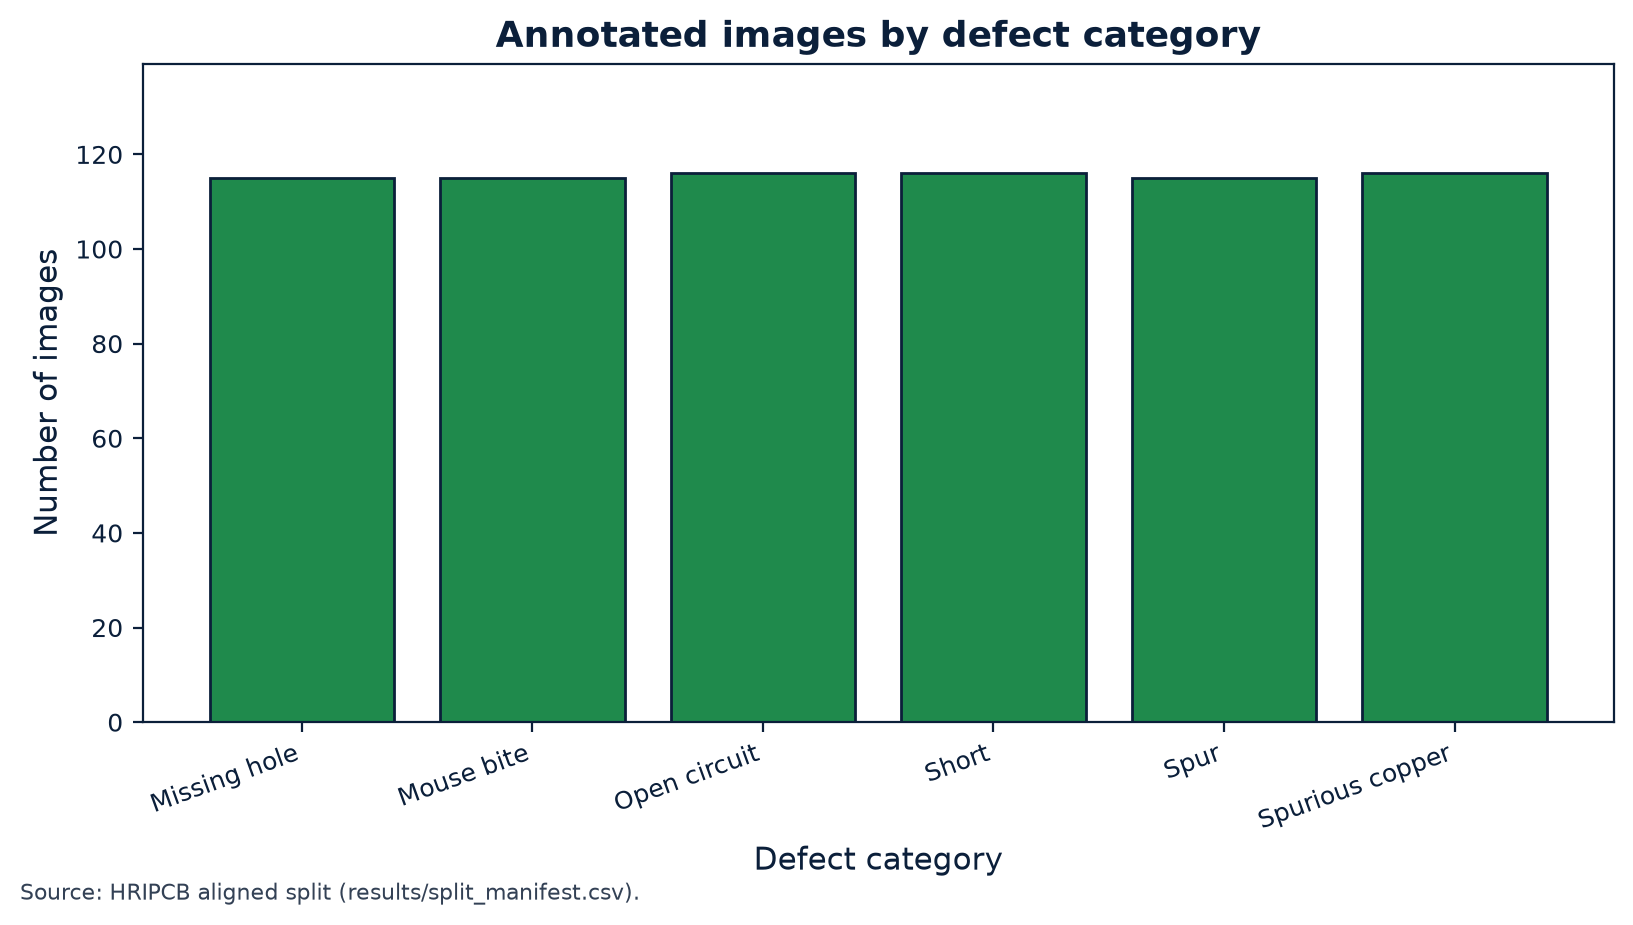
\includegraphics[width=\columnwidth]{fig01_class_distribution.png}
\caption{Annotated aligned images by class. The six classes are nearly balanced, from 115 to 116 images. Source: \texttt{results/split\_manifest.csv}.}
\label{fig:classes}
\end{figure}

\section{Threat Model and Security Assumptions}
\label{sec:threat}
The asset is a bare board that should not leave the cell with an undetected defect, together with the record of how that decision was made. The system owner sets the risk tolerance. The manufacturing operator runs the line. The quality inspector accepts or overrides the model. The model developer trains and versions the checkpoint. The supplier provides boards and, in the assumed cell, may also influence how a board is presented to the camera. The camera and lights produce the image. The inference server holds the weights and returns boxes. The audit log is the evidence that a later review can reconstruct.

The attack surfaces are the camera and lights, the acquisition and preprocessing path, the model input, the weight file, the dataset and its annotations, an inference API if one is exposed, the model output, the human approval step, monitoring, and the update path. This experiment exercises only the model input, by editing copies of test images offline. It does not modify weights, labels, or a live server.

The realistic scenarios considered are image degradation that hides a defect, a localized obstruction on the defect, a camera or fixture that presents the board at a small rotation, replacement of the weight file, corruption of training annotations, a shift after a lighting or product change, misuse of the confidence threshold, a silent monitor, and an inspector who treats the model as infallible. Likelihood and impact for the image scenarios are tied to the measurements in Section~\ref{sec:results}. The other scenarios are labeled as assessments because they were not executed.

\section{Robustness Audit Methodology}
\label{sec:method}
A detection is a true positive when its confidence is at least 0.25, its class matches the ground-truth class, and its IoU with that box is at least 0.50. Matching is one-to-one and greedy in confidence order. Precision is $TP/(TP+FP)$. Recall is $TP/(TP+FN)$. The F1 score is the harmonic mean of precision and recall. The false-negative rate is
\begin{equation}
\mathrm{FNR}=\frac{FN}{TP+FN}.
\end{equation}
When every ground-truth box is accounted for, FNR is one minus recall. Mean IoU is reported twice: over true positives only, and with each miss scored as zero. Mean confidence is reported the same way. Class consistency is counted separately by matching on IoU while ignoring class, then asking whether the predicted label differs. That count is not added to the class-aware true-positive total.

Mean average precision uses the 101-point interpolated average precision associated with the COCO evaluation tradition \cite{lin2014coco}, implemented in \texttt{calculate\_metrics.py} rather than by calling the COCO API. mAP@0.5:0.95 averages the class-wise scores at IoU thresholds $0.50,0.55,\ldots,0.95$. The percentage change requested by the proposal is
\begin{equation}
\mathrm{Percentage\ change}=\frac{M_{\mathrm{pert}}-M_{\mathrm{base}}}{M_{\mathrm{base}}}\times 100.
\end{equation}
A negative change in recall is a degradation. A positive change in FNR is also a degradation.

Each test image is copied before it is modified. The families and the three intensity levels are brightness offsets $-40,+40,+80$; contrast factors $0.6,0.8,1.4$; Gaussian blur kernels $3,9,15$; Gaussian noise standard deviations $10,25,40$; JPEG qualities $75,40,15$; rotations of $3,7,12$ degrees; scales $0.85,1.15,1.30$; horizontal illumination gradients of strength $0.25,0.45,0.65$; and centered gray occlusions whose side length is $0.30,0.55,0.80$ of each ground-truth box. The side fraction is not an area fraction. A side fraction of 0.55 covers $0.55^{2}\approx 30$ percent of the box area. Geometric transforms rewrite the boxes. Photometric transforms and occlusion keep the original boxes, because the question is whether the detector still finds a defect that the annotation still marks. Occlusion is a sensitivity test. It is not an optimized adversarial patch, and it is not claimed to transfer to a factory camera.

Risk score is likelihood times impact, each an integer from 1 to 5. For an image threat, likelihood is taken from the recall drop at intensity level 2: drop below 0.05 maps to 2, below 0.15 maps to 3, below 0.30 maps to 4, and a larger drop maps to 5. Impact is an engineering judgment about a missed bare-board defect, not a measured warranty cost. Scores of 1--6, 7--12, 13--19, and 20--25 are labeled Low, Medium, High, and Critical. A control that addresses a risk is not described as removing it.

\section{Experimental Results}
\label{sec:results}
\subsection{Baseline}
On the 108 clean test images, class-aware matching at the operating point yields 428 true positives, 35 false positives, and 49 false negatives. Precision is 0.924, recall is 0.897, F1 is 0.911, and the false-negative rate is 0.103. mAP@0.5 is 0.921 and mAP@0.5:0.95 is 0.455. The gap between those two mAP numbers means many accepted boxes clear IoU 0.50 but do not remain well aligned as the threshold rises toward 0.95. Mean IoU of the true positives is 0.760. Mean confidence, with misses scored as zero, is 0.620. Figure~\ref{fig:baseline} summarizes the operating point.

\begin{figure}[t]
\centering
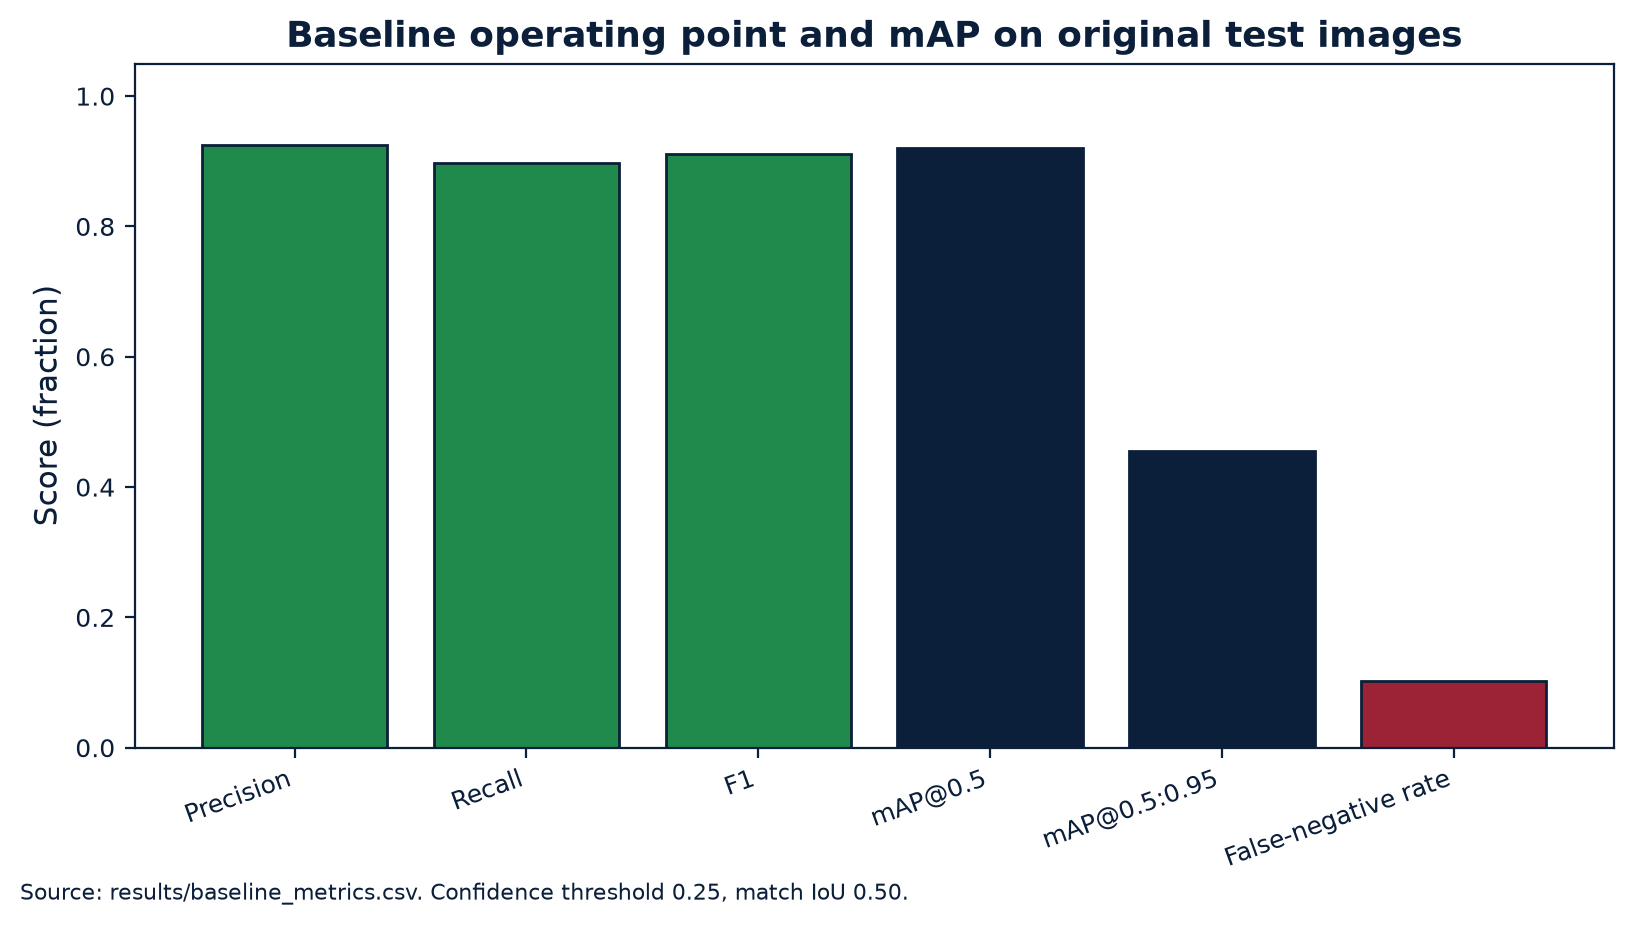
\includegraphics[width=\columnwidth]{fig02_baseline_metrics.png}
\caption{Baseline on unmodified test images. mAP@0.5 is close to recall. mAP@0.5:0.95 is much lower, so localization is the weaker of the two detection qualities. Source: \texttt{results/baseline\_metrics.csv}.}
\label{fig:baseline}
\end{figure}

\begin{table}[t]
\caption{Class-aware baseline on the test split}
\label{tab:perclass}
\centering
\footnotesize
\begin{tabular}{lrrrr}
\toprule
Class & Boxes & Recall & FNR & AP@0.5 \\
\midrule
Missing hole & 82 & 0.988 & 0.012 & 0.990 \\
Mouse bite & 76 & 0.842 & 0.158 & 0.918 \\
Open circuit & 78 & 0.833 & 0.167 & 0.878 \\
Short & 83 & 0.988 & 0.012 & 0.964 \\
Spur & 81 & 0.864 & 0.136 & 0.897 \\
Spurious copper & 77 & 0.857 & 0.143 & 0.880 \\
\bottomrule
\end{tabular}
\end{table}

Table~\ref{tab:perclass} shows that missing holes and shorts are already easier than mouse bites, open circuits, spurs, and spurious copper before any perturbation. Class-agnostic IoU matching produces 434 overlaps, of which 7 have the wrong class, plus 43 misses and 29 false positives. The class-aware false-negative count is 49 rather than 43 because a wrong-class overlap is not a true positive. Wrong class is real but uncommon. The usual clean-image error is a miss or an extra box, not a relabeling of a found defect.

\subsection{Perturbations}
Figure~\ref{fig:recall} and Figure~\ref{fig:fnr} are the main robustness results. Table~\ref{tab:recall} lists recall at all three levels. Three families move the detector. Six do not, at the intensities tested.

\begin{figure*}[t]
\centering
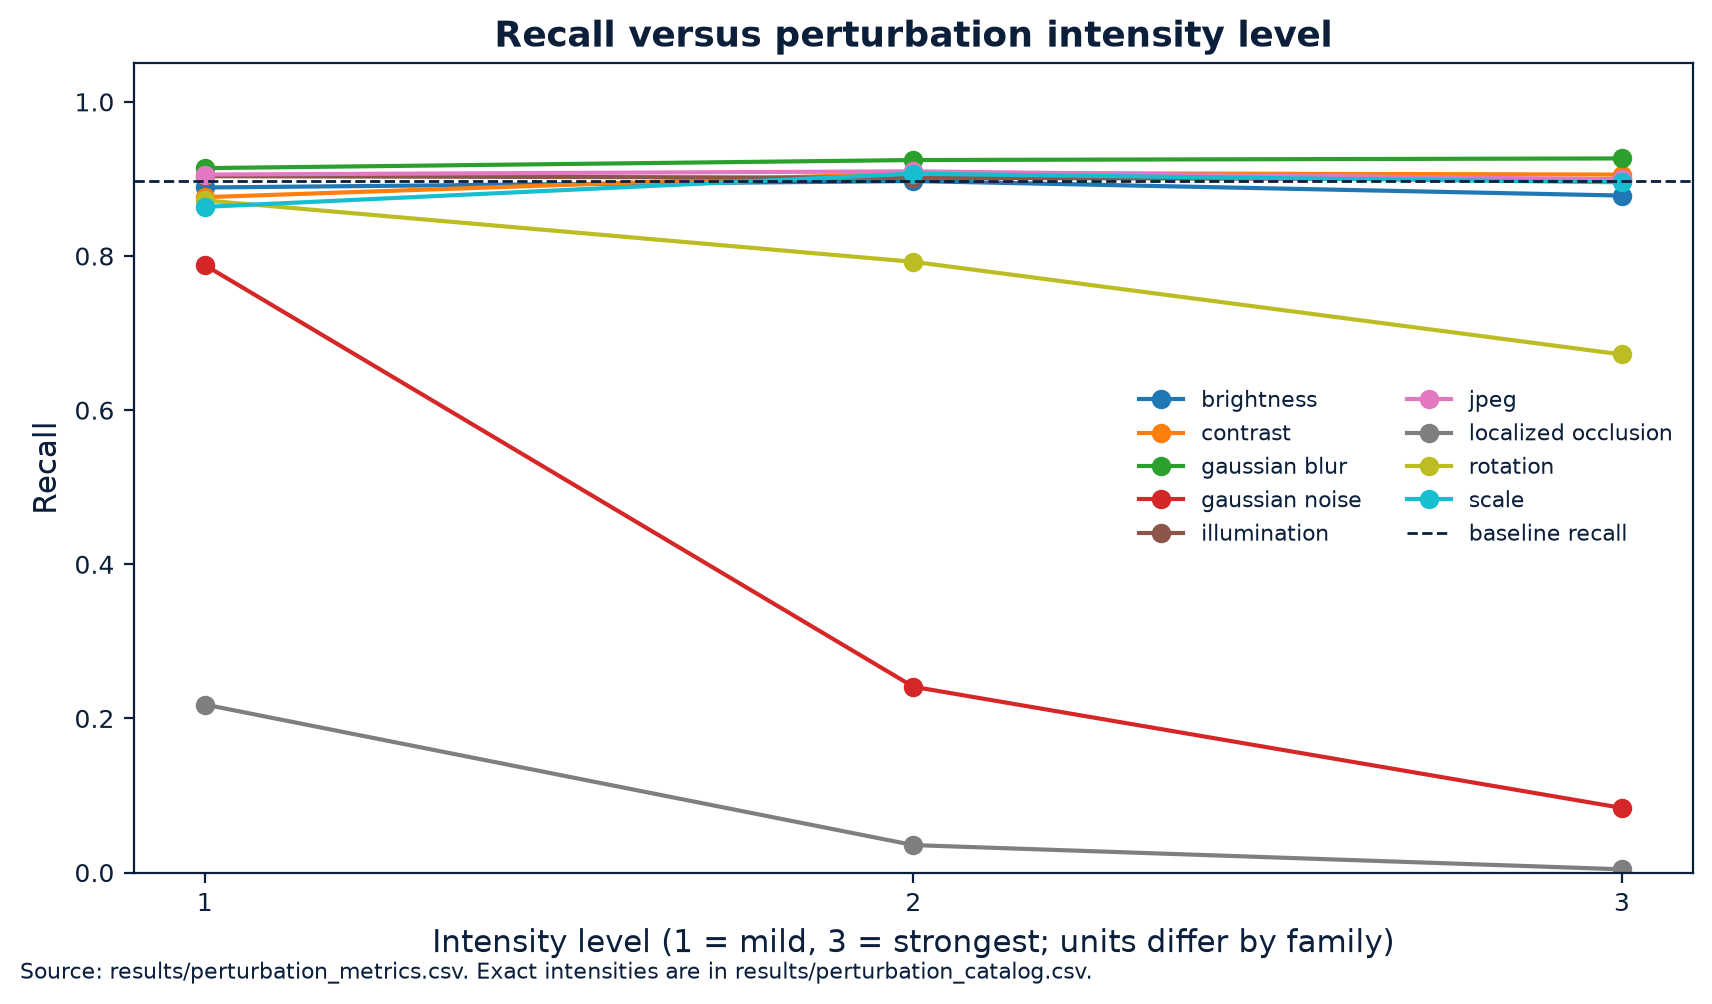
\includegraphics[width=0.92\textwidth]{fig03_recall_vs_intensity.png}
\caption{Recall against intensity level. Noise, centered occlusion, and rotation leave the baseline. Blur stays slightly above it. The horizontal axis is a level index because the physical units differ; the units are listed in Section~\ref{sec:method}. Source: \texttt{results/perturbation\_metrics.csv}.}
\label{fig:recall}
\end{figure*}

\begin{figure*}[t]
\centering
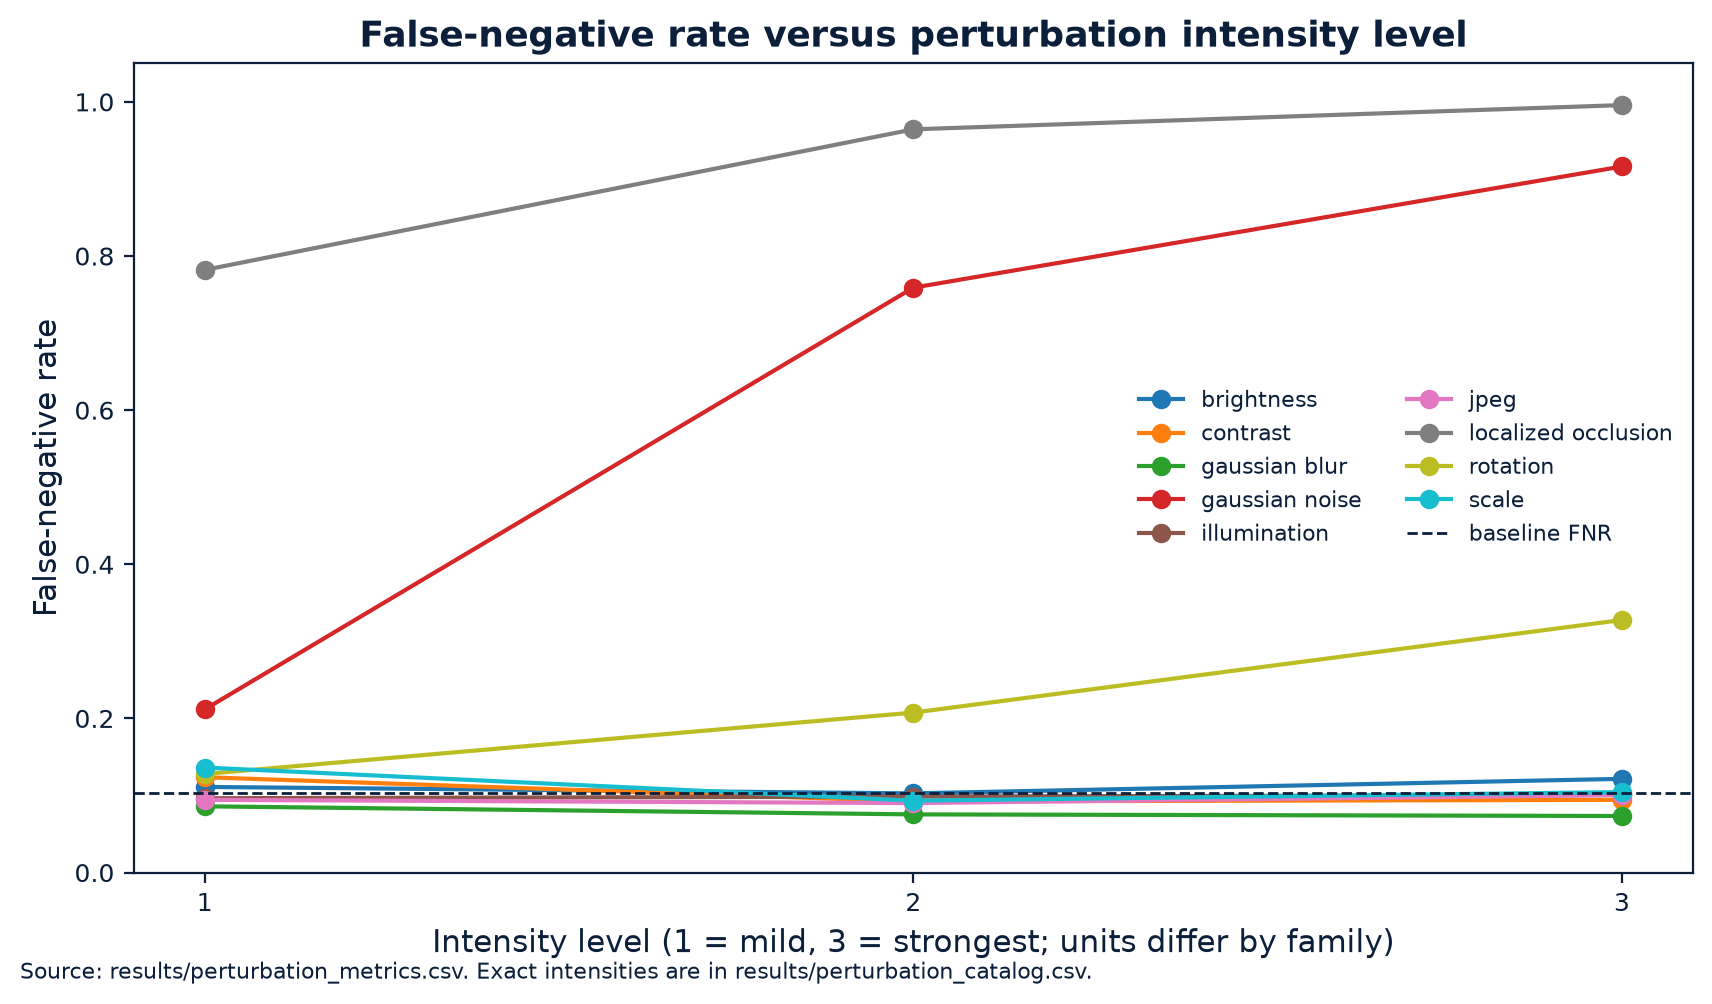
\includegraphics[width=0.92\textwidth]{fig04_fnr_vs_intensity.png}
\caption{False-negative rate against the same intensity levels. The curves invert Figure~\ref{fig:recall}, which is expected because FNR is one minus recall when the ground-truth count is unchanged. Rotation at 12 degrees and the larger scales change that count slightly, as discussed in the text. Source: \texttt{results/perturbation\_metrics.csv}.}
\label{fig:fnr}
\end{figure*}

\begin{table}[t]
\caption{Test recall by family and intensity level}
\label{tab:recall}
\centering
\footnotesize
\begin{tabular}{lccc}
\toprule
Family & Level 1 & Level 2 & Level 3 \\
\midrule
Brightness & 0.889 & 0.897 & 0.878 \\
Contrast & 0.876 & 0.908 & 0.906 \\
Gaussian blur & 0.914 & 0.925 & 0.927 \\
Gaussian noise & 0.788 & 0.241 & 0.084 \\
Illumination & 0.904 & 0.901 & 0.899 \\
JPEG & 0.906 & 0.910 & 0.899 \\
Occlusion & 0.218 & 0.036 & 0.004 \\
Rotation & 0.872 & 0.792 & 0.672 \\
Scale & 0.864 & 0.907 & 0.896 \\
\bottomrule
\end{tabular}
\end{table}

Noise is the severe photometric failure. At standard deviations 10, 25, and 40, recall is 0.788, 0.241, and 0.084. The level-2 percentage change in recall is $-73.1$ percent, and the false-negative rate rises from 0.103 to 0.759. mAP@0.5 falls from 0.921 to 0.259. At level 2, missing-hole recall remains 0.866, while spur recall falls to 0 and spurious-copper recall falls to 0.013. The large dark hole survives moderate noise. The thin copper defects do not. Standard deviation 40 is a harsh noise level, not a subtle one. The result says the frozen detector has little margin once high-frequency noise becomes strong. It does not say that every factory camera produces that noise.

Centered occlusion is the other severe condition, and it should be read for what it is. Covering 9 percent of each box area (side fraction 0.30) drops recall to 0.218. Covering about 30 percent of the area (side fraction 0.55) drops recall to 0.036, a $-96.0$ percent change. Covering 64 percent of the area drops recall to 0.004. At the middle level, only spur retains any recall, and that recall is 0.210. The few boxes that remain true positives are still reasonably localized: mean IoU among those true positives at level 2 is 0.818, while mean IoU with misses scored as zero collapses. The detector does not infer a covered defect from the surrounding copper. That is operationally relevant for tape, a smear, or a mark placed on the defect. It is not evidence for the Lee--Kolter phenomenon, in which a patch suppresses objects it does not cover \cite{lee2019patch}. Figure~\ref{fig:panel} shows one missing hole before and after the middle occlusion and the middle noise level.

\begin{figure}[t]
\centering
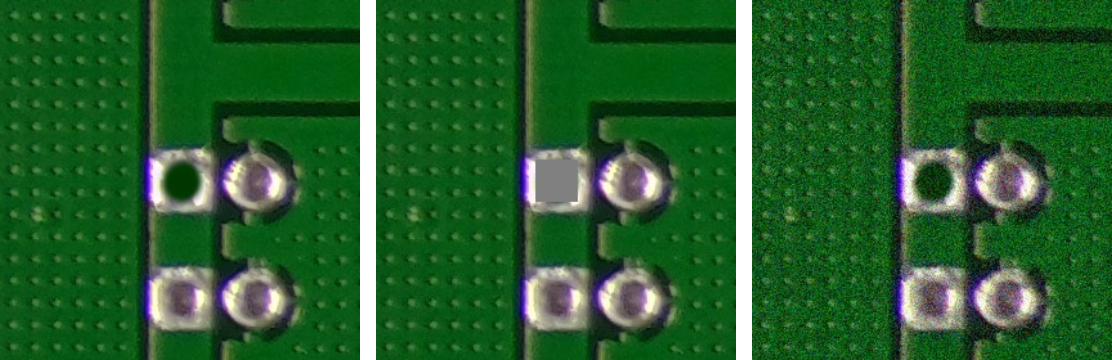
\includegraphics[width=\columnwidth]{examples/comparison_panel.png}
\caption{One missing hole from test image \texttt{01\_missing\_hole\_09}. Left: original. Center: gray occlusion at side fraction 0.55. Right: Gaussian noise at standard deviation 25. The crop uses the original box. Rotation is not shown here because the defect moves and the original crop would be misleading.}
\label{fig:panel}
\end{figure}

Rotation is the geometric failure. Recall is 0.872 at 3 degrees, 0.792 at 7 degrees ($-11.7$ percent), and 0.672 at 12 degrees ($-25.1$ percent). mAP@0.5 at 12 degrees is 0.659. One box leaves the canvas at 12 degrees, so the denominator is 476 rather than 477. Missing-hole recall at 12 degrees stays at 0.976. Spur recall falls to 0.432. Training used no rotation augmentation, which is a plausible reason for this gap. Scale at 0.85 lowers recall only to 0.864. Scales 1.15 and 1.30 keep recall near the baseline, but they also crop boxes out of the frame: 472 and 431 ground-truth boxes remain. Those lost boxes are an acquisition failure even though the recall of the surviving boxes looks acceptable. A quality gate has to count boards that no longer fit the field of view, not only the recall of what remains.

Brightness, contrast, illumination, and JPEG quality down to 15 leave recall between 0.876 and 0.910. Blur kernels 3, 9, and 15 raise recall slightly, to 0.914, 0.925, and 0.927. The proposal expected blur to hurt small defects. On these images it did not. A 15-pixel kernel on a roughly 3{,}000-pixel-wide photograph is only a few pixels after the network letterboxes the image to 640. The tested blur is mild at the tensor the detector sees. A stronger blur, or blur applied after resizing, is untested. Figure~\ref{fig:map} shows the same split in mAP@0.5. Figure~\ref{fig:heat} shows that the clean-image advantage of missing holes largely survives noise and rotation and disappears under occlusion.

\begin{figure}[t]
\centering
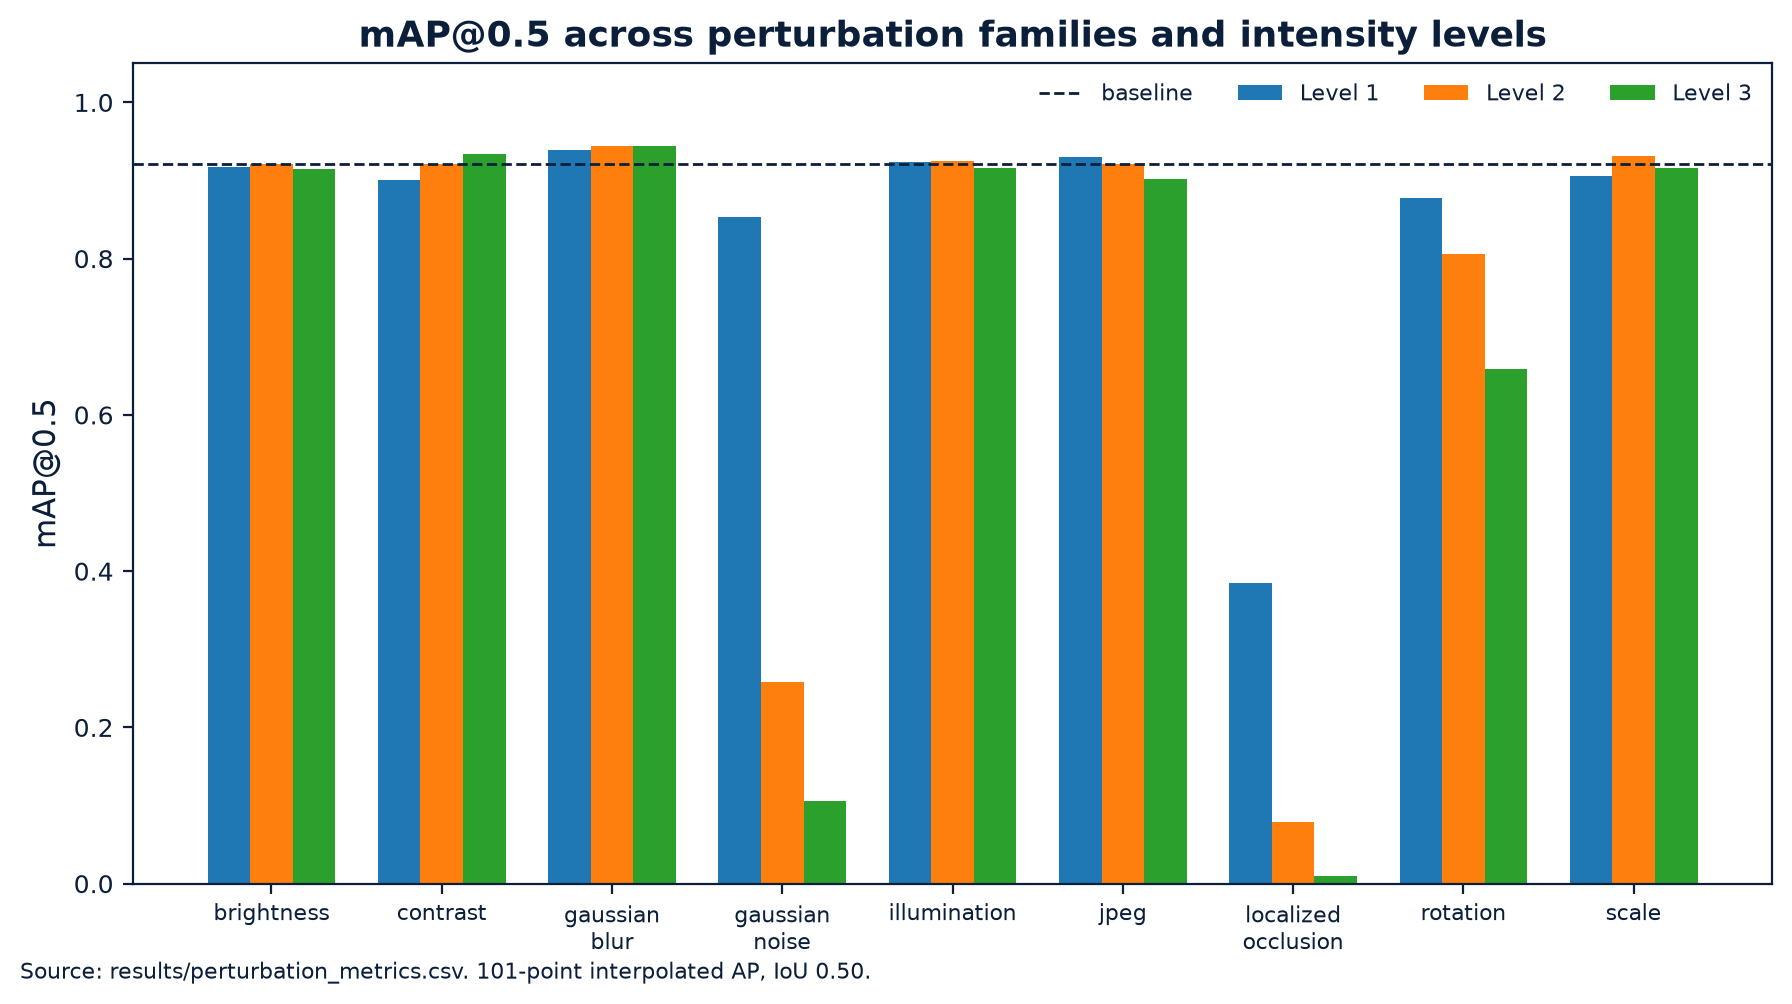
\includegraphics[width=\columnwidth]{fig05_map_by_perturbation.png}
\caption{mAP@0.5 by family and level. The pattern matches recall: noise and occlusion fall, rotation falls more slowly, and the global photometric families stay near the baseline. Source: \texttt{results/perturbation\_metrics.csv}.}
\label{fig:map}
\end{figure}

\begin{figure*}[t]
\centering
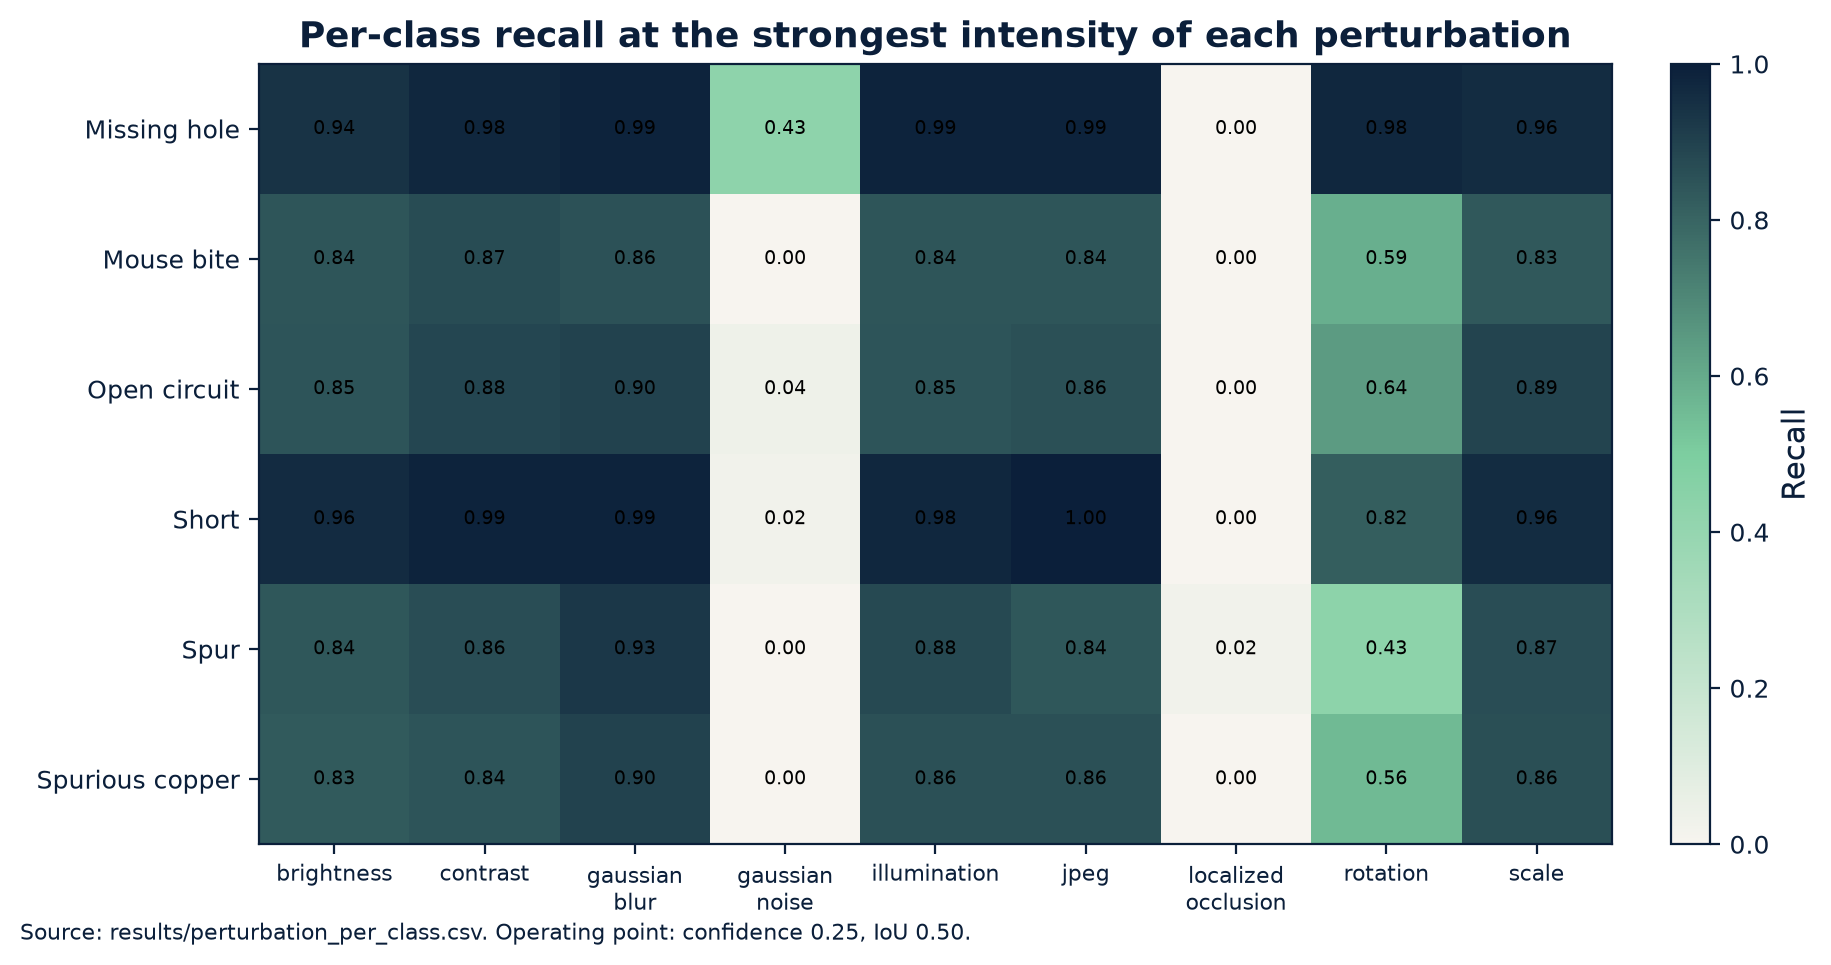
\includegraphics[width=0.92\textwidth]{fig08_class_robustness_heatmap.png}
\caption{Per-class recall at the strongest level of each family. Missing holes remain detectable under strong noise and a 12-degree rotation. They are not detectable when the hole itself is covered. Spur is the fragile class under both noise and rotation. Source: \texttt{results/perturbation\_per\_class.csv}.}
\label{fig:heat}
\end{figure*}

Confidence and IoU follow the misses. With misses scored as zero, mean confidence falls from 0.620 on clean images to 0.147 under noise level 2 and to 0.015 under occlusion level 2. Mean IoU scored the same way falls to 0.173 and 0.026. The charts of those two series are \texttt{fig06} and \texttt{fig07} in the project figures directory. They are not independent failure modes. They fall because the detector emits nothing, and the metric then inserts a zero. Where a detection survives, its IoU does not show a separate large localization collapse except under the 12-degree rotation, where mean IoU of the remaining true positives is 0.712 against a clean-image 0.760.

The practical reading is narrower than ``the model is fragile to the factory.'' On this checkpoint and this test split, clean-image mAP@0.5 of 0.921 coexists with a large miss rate under strong noise, under a patch that hides the defect, and under a rotation the training recipe never showed the model. Global exposure and moderate JPEG compression are not, by themselves, the observed problem.

\section{MITRE ATLAS Threat Mapping}
\label{sec:atlas}
Technique names, identifiers, and descriptions are taken from ATLAS content 2026.10 \cite{mitre2026atlas}. Tactic placement is taken from the tactic lists in the distributed ATLAS matrix (version 5.6.0), whose identifiers still match the 2026.10 technique records. The 2026.10 technique objects used for the wording do not repeat that tactic array, so the tactic column is cited at that older matrix version. AML.T0076, ``Corrupt AI Model,'' is intentionally unused. In the 2026.10 text it means damaging a file so that a model scanner fails during deserialization. It is not the name for replacing a production checkpoint.

\begin{table*}[t]
\caption{ATLAS techniques and the kind of evidence attached to each}
\label{tab:atlas}
\centering
\footnotesize
\setlength{\tabcolsep}{4pt}
\begin{tabular}{@{}>{\raggedright\arraybackslash}p{0.13\textwidth}>{\raggedright\arraybackslash}p{0.34\textwidth}>{\raggedright\arraybackslash}p{0.48\textwidth}@{}}
\toprule
ID & Name and tactic & Evidence in this audit \\
\midrule
AML.T0043 & Craft Adversarial Data; AI Attack Adaptation. Sub-technique AML.T0043.003, Manual Modification. & Demonstrated as a laboratory input edit. Noise, rotation, and gray occlusion change detections. This is not an optimized attack. \\
AML.T0015 & Evade AI Model; Impact. Also listed under Initial Access and Defense Evasion for other uses. & Plausible consequence. A miss is the inspection analogue of a missed detection. No factory system was evaded. \\
AML.T0041 & Physical Environment Access; AI Model Access. & Literature and scenario \cite{eykholt2018physical,lee2019patch}. The edits were digital. \\
AML.T0042 & Verify Attack; AI Attack Adaptation. & The evaluators did this offline, on their own copy, as the audit method. It was not done against a victim API. \\
AML.T0040 & AI Model Inference API Access; AI Model Access. & Scenario only. No networked API was exposed. \\
AML.T0044 & Full AI Model Access; AI Model Access. & Scenario only. The checkpoint is a local file. It was not stolen. \\
AML.T0018 & Manipulate AI Model; Persistence. Sub-technique AML.T0018.000, Poison AI Model. & Scenario only. Weights were not edited after training. \\
AML.T0020 & Training Data Poisoning; Resource Development and Persistence. & Scenario only. The training split was not poisoned. \\
AML.T0059 & Erode Dataset Integrity; Impact. & Scenario only. Labels were not corrupted. \\
AML.T0031 & Erode AI Model Integrity; Impact. & Plausible if the measured degradation were left unmonitored. Not demonstrated as a campaign. \\
AML.T0010 & Supply Chain Compromise; Initial Access. Sub-technique AML.T0010.003, Model Repository. & Scenario only. The public pretrained file was not replaced. \\
\bottomrule
\end{tabular}
\end{table*}

Table~\ref{tab:atlas} is the mapping. Official pages are \url{https://atlas.mitre.org/techniques/} followed by the identifier. ATLAS mitigations that match the plan below, without being claimed as complete, are AML.M0015 (Predictive AI Adversarial Input Detection), AML.M0003 (Predictive AI Model Hardening), AML.M0009 (Predictive AI Multi-Sensor Fusion), AML.M0005 (Control Access to AI Models and Data at Rest), AML.M0014 (Verify AI Artifacts), and AML.M0007 (Sanitize Training Data) \cite{mitre2026atlas}.

\section{Governance Risk Assessment}
\label{sec:gov}
The assessment follows the four NIST functions \cite{nist2023airmf,nist2023playbook}.

\textbf{Govern.} A bare-board model is a decision-support component. The quality manager owns the accept rule. The model developer does not change the threshold alone. Missing-hole, open-circuit, and short defects are treated as higher consequence than a cosmetic copper nick because they change connectivity. That ranking is a judgment.

\textbf{Map.} The context is the assumed cell in Section~\ref{sec:system}. The measured hazards are strong noise, obstruction of the defect, and untrained rotation. The unmeasured hazards are weight substitution, label damage, and an unreviewed process change. Clean mAP is not the context.

\textbf{Measure.} The evidence is the frozen test comparison. For release, the relevant tests are noise at standard deviation 25, occlusion at side fraction 0.55, and rotation at 7 and 12 degrees, reported per class. Blur at a 15-pixel kernel is not a sufficient robustness test for this image size.

\textbf{Manage.} Boards are held, not auto-accepted, when the image-quality gate fails or when confidence collapses. The last signed checkpoint is the rollback target. A lighting, lens, fixture, or board-family change reopens validation. None of these actions drives the measured recall drop to zero.

Figure~\ref{fig:risk} places the ten register rows. R1 (noise) and R2 (occlusion) are Critical because level-2 recall collapses and the impact judgment is 4. R5 (rotation) is Medium. R3 (brightness) and R4 (JPEG) are Low because the level-2 recall drop is below 0.05. R6 through R10 remain scenario assessments: weight modification is High on a high impact judgment, not because an edit was performed. The register is \texttt{results/risk\_register.csv}.

\begin{figure}[t]
\centering
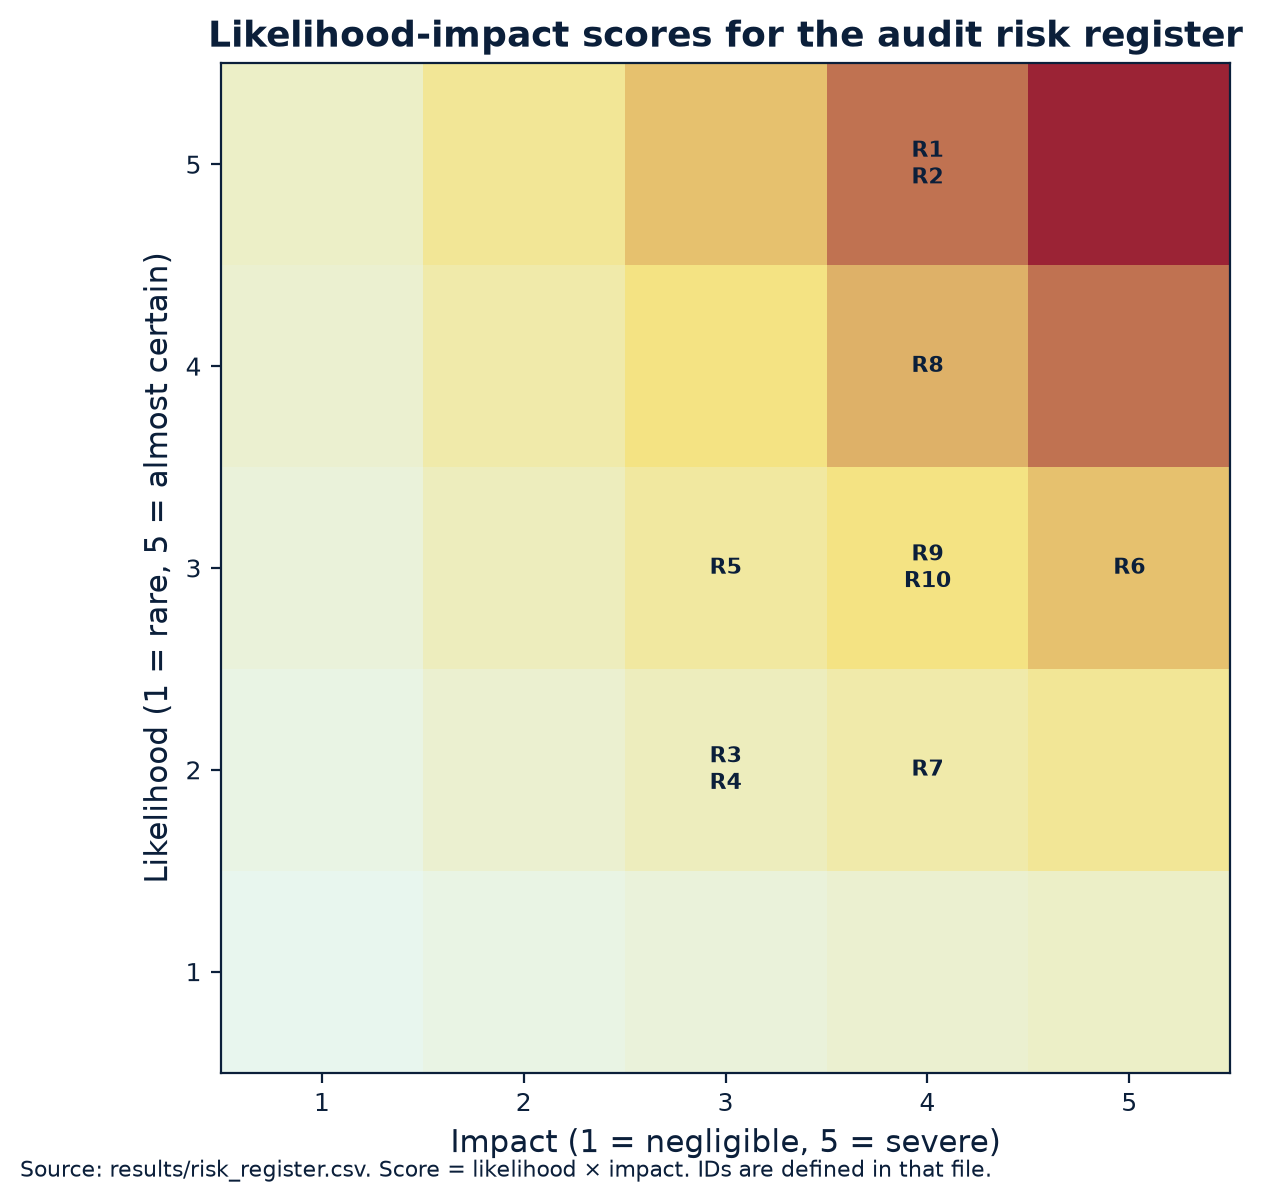
\includegraphics[width=\columnwidth]{fig10_risk_heatmap.png}
\caption{Likelihood-impact grid. Identifiers that share a cell are stacked. R1 and R2 are the measured critical cells. R6--R10 are judgments, not experiment outputs. Source: \texttt{results/risk\_register.csv}.}
\label{fig:risk}
\end{figure}

\section{Controls and Assurance Plan}
\label{sec:controls}
The plan below is what the assumed cell can implement. It is not a claim that the controls were deployed, and it is not a claim that residual risk is gone.

Before deployment, the organization records the checkpoint hash, the class list, the confidence and NMS thresholds, the training-split identifier, and the image-size range. Annotation review samples new labels before they enter training. The release test repeats the clean test and the three degrading conditions. An image is rejected before inference when its noise, resolution, or board angle is outside the validated window, or when the board does not fill the expected field of view. The running monitor tracks confidence, per-class recall on a labeled audit sample, and the false-negative rate of that sample. A low-confidence board, a class with a rising miss rate, or an out-of-window image goes to a person. The person can accept, rework, or hold. Skipping that review is itself an incident.

Logs store the image identifier, the weight hash, the threshold, the boxes and confidences, the quality-gate result, the reviewer's decision, and the time. Model version and data version move together. A camera, light, PCB family, or software change triggers revalidation rather than a silent continuation. Safety-relevant classes, in this judgment the open, short, and missing-hole classes, keep a second look, either a second algorithm or a human sample, because the detector's clean recall on mouse bites and open circuits is already below the recall on missing holes. The minimum release bar suggested by this audit is clean test recall of at least 0.85 on every class, noise-level-2 recall drop no greater than 0.10 on every class, and occlusion treated as a hold condition rather than as a case the model is expected to solve. The present checkpoint does not meet the noise bar. Residual risk is accepted in writing by the quality manager, with a review date, or the model stays out of automatic accept.

Table~\ref{tab:assure} is the measured part of the assurance matrix. The full matrix, including the scenario rows, is \texttt{tables/assurance\_matrix.csv}. Figure~\ref{fig:cover} shows which controls are relevant to which risks. A filled cell means the control is aimed at that risk. It does not mean the control was tested in production or that the risk is closed.

\begin{table}[t]
\caption{Assurance actions tied to measured risks}
\label{tab:assure}
\centering
\scriptsize
\setlength{\tabcolsep}{3pt}
\begin{tabular}{@{}>{\raggedright\arraybackslash}p{0.18\columnwidth}>{\raggedright\arraybackslash}p{0.40\columnwidth}>{\raggedright\arraybackslash}p{0.38\columnwidth}@{}}
\toprule
Risk & Acceptance evidence & If it fails \\
\midrule
R1 noise & Level-2 recall drop $\le 0.10$ on each class & Do not auto-accept; fix the sensor path or retrain \\
R2 occlusion & Any centered cover at side fraction 0.55 holds the board & Human review; do not expect the model to see through the cover \\
R5 rotation & Level-2 recall drop $\le 0.10$ & Correct the fixture and revalidate \\
R3, R4 & Keep the photometric replay, but do not treat a pass as general robustness & Investigate only if a future level-2 drop exceeds 0.10 \\
\bottomrule
\end{tabular}
\end{table}

\begin{figure}[t]
\centering
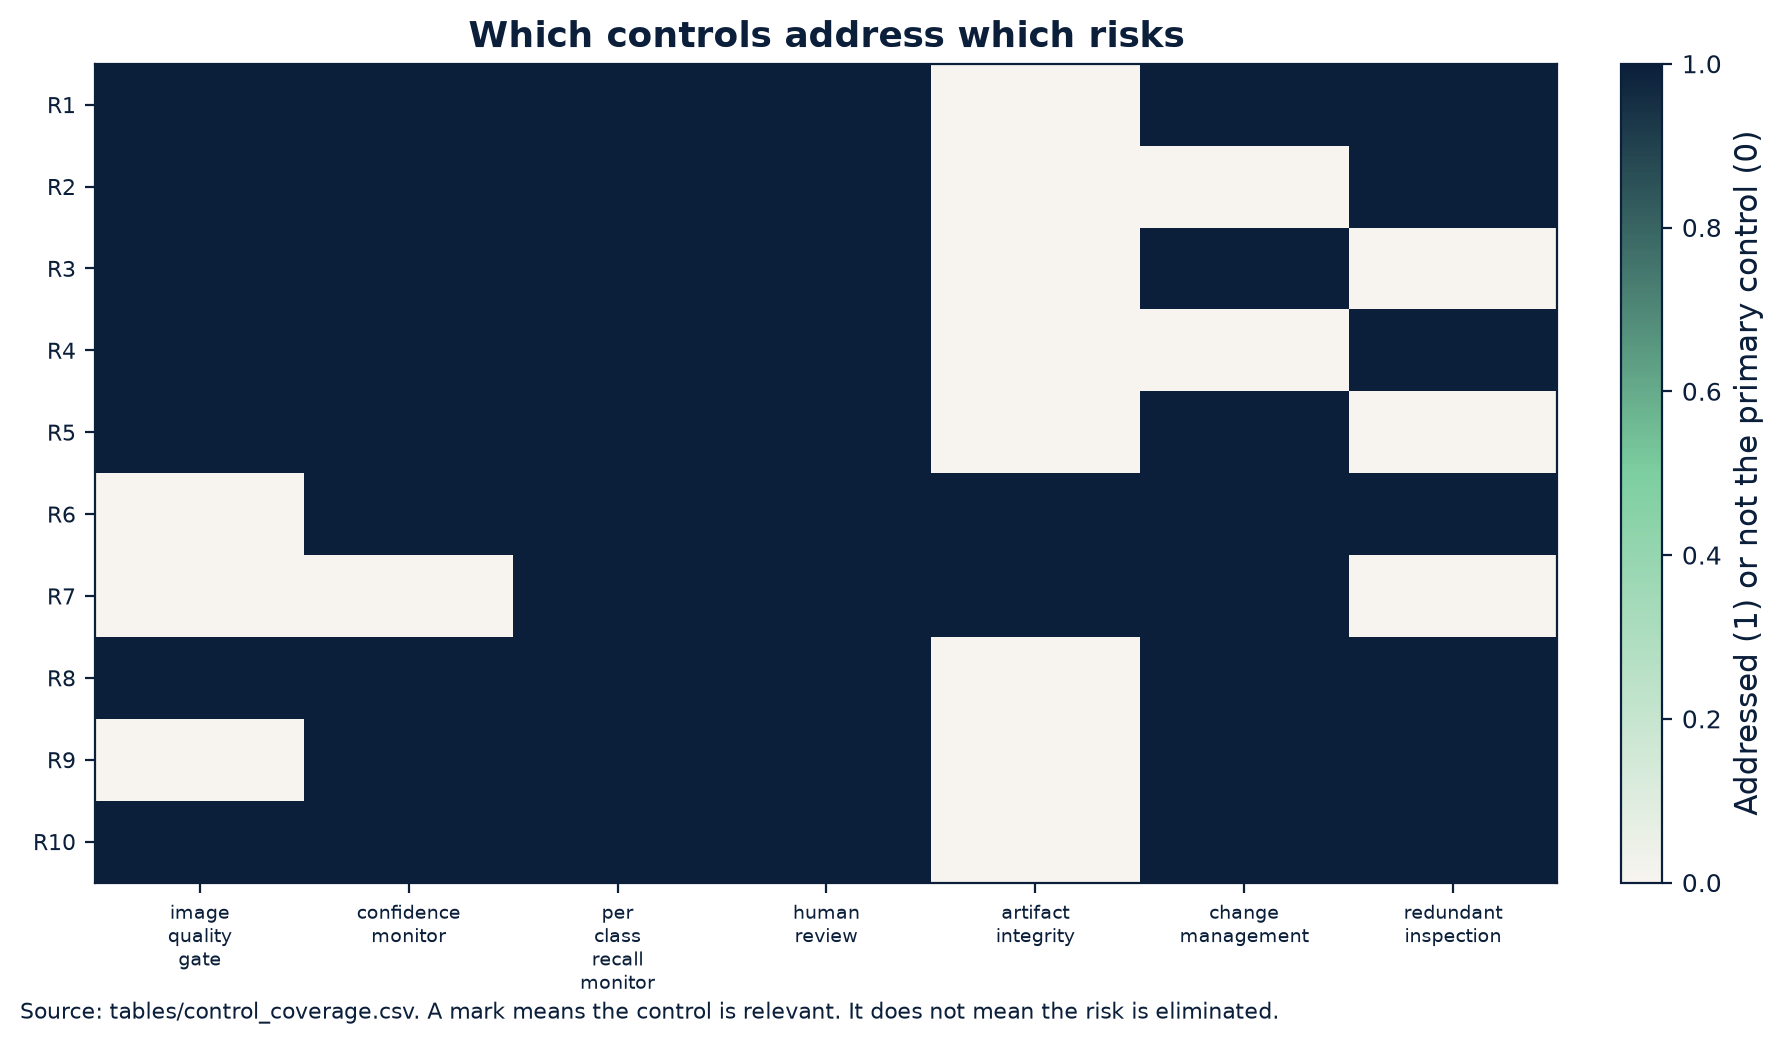
\includegraphics[width=\columnwidth]{fig12_control_coverage.png}
\caption{Control coverage. Image-quality, confidence, recall, and human review address the measured input risks. Artifact integrity addresses weight and data risks that this experiment did not execute. Source: \texttt{tables/control\_coverage.csv}.}
\label{fig:cover}
\end{figure}

\section{Limitations and Ethical Considerations}
The images are synthesized research images \cite{huang2020hripcb}. They do not represent every camera, finish, or defect distribution in manufacturing. The rotated half of HRIPCB was excluded. Thirty epochs produced a usable detector, but the clean mAP is not the 98--99 percent reported by longer, different training runs \cite{niu2023yolov5,xiao2024cdiyolo}, and the architecture is YOLOv5u-s rather than the older anchor-based YOLOv5s those papers usually mean. Blur and JPEG were mild after the 640-pixel letterbox. Noise at standard deviation 25 and 40 is obvious to a person. Occlusion hides the defect on purpose, so the recall collapse is evidence of dependence on local appearance, not of a transferable physical patch attack. Impact scores are judgments. One split and one checkpoint cannot support a claim about all PCB detectors. The mAP code was checked on a perfect detection and on a total miss; it was not cross-certified with the COCO evaluation tool.

The work used a public dataset, offline, on copies of the test images. It does not provide a procedure for hiding defects on a production line, for optimizing a physical patch, or for altering another organization's model. The gray rectangle is a laboratory probe. Using it, or the noise script, against a system the evaluator does not own would be outside this authorization.

\section{Future Work}
A next audit would add the rotated HRIPCB images only after the boxes are transformed with the published angles, test blur after letterboxing, and compare this checkpoint with an anchor-based YOLOv5s trained in the original repository \cite{jocher2020yolov5}. A physical trial needs a camera, a fixture, and permission from the line owner. It is not a substitute for the controls in Section~\ref{sec:controls}. Per-class noise augmentation is a model-hardening experiment worth running because missing holes and spurs did not fail together. That experiment is future work; it was not done here.

\section{Conclusion}
The frozen YOLOv5u-s prototype finds 89.7 percent of the 477 defects on clean HRIPCB test images and reaches mAP@0.5 of 0.921. That benchmark does not survive strong additive noise, a gray cover on the defect, or a rotation of about 7 to 12 degrees. It does survive the tested brightness, contrast, illumination, JPEG, mild blur, and mild scale changes, with the caveat that aggressive scaling pushes defects out of the frame. Class swaps are uncommon. The governance implication is specific. An organization that auto-accepts boards from this class of detector needs a noise and geometry gate, a hold rule when the defect region is obstructed, per-class miss monitoring, signed weights, and a person on the low-confidence path. Clean accuracy is the starting measurement, not the release decision.

\FloatBarrier
\bibliographystyle{IEEEtran}
\bibliography{references}

\end{document}
